% !TEX root = ../presentation.tex
% !BIB program = biber
% !TEX program = xelatex

\section{Introduction}


\begin{frame}
    \frametitle{Healthcare}
    \begin{quotation}
        \noindent\centering
        Healthcare is the improvement of health via the {\color{dtured}prevention}, {\color{dtured}diagnosis}, {\color{dtured}treatment}, {\color{dtured}amelioration} or {\color{dtured}cure} of {\color{theme-green}disease}, {\color{theme-green}illness}, {\color{theme-green}injury}, and {\color{theme-green}other physical and mental impairments} in people.
    \end{quotation}
\end{frame}


\begin{frame}
    \frametitle{Medical dialogue}
    \begin{figure}
        \centering
        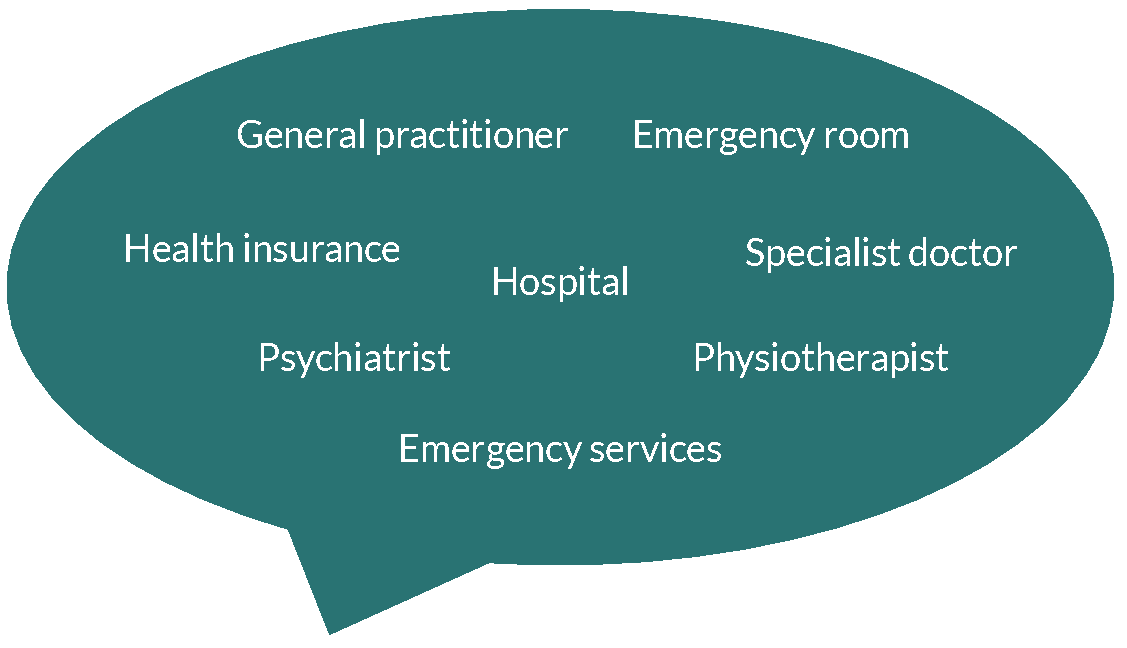
\includegraphics[width=0.7\paperwidth]{figures/speech_bubble.pdf}
    \end{figure}

    \note[item]{Healthcare sector is a complex system}
\end{frame}


\begin{frame}
    \frametitle{Errors in medical dialogue}
    \begin{itemize}
        \item<1,2>Communication is everywhere in healthcare. 
        \item <1,2>It is complex, involving multiple participants, different contexts, and different purposes.
        \item <2> {\color{dtured} } Failure of communication is a leading cause of medical error contributing to two out of three adverse events \cite{starmer_changes_2014}.
        \item <2> A considerable fraction of all hospital admissions had preventable adverse outcomes (9\% to 16.6\% in AU, NZ, UK, DK) \cite{carver_medical_2024}.
    \end{itemize}
\end{frame}


% \begin{frame}
%     \frametitle{Types of dialogue}
%     \begin{itemize}
%         \item Domain: Specialized / General
%         \item Context: Controlled / Chaotic
%         \item Person: Nurse, doctor, midwife, caregiver, psychiatrist, insurance professional
%         \item Purpose: Triaging, diagnosis, treatment, follow-up, documentation, coding, billing
%     \end{itemize}
% \end{frame}



\begin{frame}
    \frametitle{Documenting medical encounters}
    \begin{itemize}
        \item <1,2> Documentation is a central part of healthcare.
        \item <1,2> E.g. patient records, insurance claims, billing, research, training, legal purposes.
        \vspace{1em}
        \item <2> {\color{dtured}Time}: Physicians spend 34-37\% of their time on documentation \cite{joukes_time_2018, tipping_where_2010, sinsky_allocation_2016}\footnote{Ambulatory care across four specialties in four states and tertiary care at an academic medical center.}.
        \item <2> {\color{dtured}Quality}: Discharge summaries rarely meet all timeline, transmission, and content criteria. \cite{horwitz_comprehensive_2013}\footnote{Outpatient visits, Yale-New Haven Hospital.}
    \end{itemize}
    
    \note[item]{Documentation is essential for a number of purposes but is very time-consuming and imperfect}
\end{frame}


\begin{frame}
    \frametitle{How might machine learning help?}
    \begin{itemize}
        \item <1> {\color{dtured}Assist} with documentation.
        \item <1> {\color{dtured}Augment} communication.
        \item <1> {\color{dtured}Improve} decision-making.
        \vspace{1em}
        \item <1> {\color{dtured}Reduce} errors.
        \item <1> {\color{dtured}Save} time.
    \end{itemize}
\end{frame}


\begin{frame}
    \frametitle{Reliability of machine learning}
    \begin{itemize}
        \item <1> {\color{dtured}Data}: Privacy, quality, quantity, diversity.
        \item <1> {\color{dtured}Interpretability}: Trust, ethics, regulation.
        \item <1> {\color{dtured}Explainability}: Transparency, accountability.
        \item <1> {\color{dtured}Robustness}: Adversarial attacks, distribution shift.
        \item <1> {\color{dtured}Bias}: Fairness, transparency.
        \item <1> {\color{dtured}Complexity}: Context, domain, language, culture.
    \end{itemize}

    

\end{frame}

